\documentclass[12pt]{article}
\usepackage{amsmath,amssymb,amsthm,mathtools,bm}
\usepackage[authoryear]{natbib}
\usepackage{graphicx,booktabs,enumitem}
\usepackage{algorithm,algpseudocode}
\usepackage[hidelinks]{hyperref}
\usepackage{xr-hyper}
\externaldocument[S-]{supplement}

% ASA template conventions -------------------------------------------------
\newcommand{\blind}{0}
\addtolength{\oddsidemargin}{-.5in}
\addtolength{\evensidemargin}{-1in}
\addtolength{\textwidth}{1in}
\addtolength{\textheight}{1.7in}
\addtolength{\topmargin}{-1in}
\newcommand{\spacingset}[1]{\renewcommand{\baselinestretch}{#1}\small\normalsize}
\spacingset{1}

\renewcommand{\topfraction}{0.9}\renewcommand{\bottomfraction}{0.8}\renewcommand{\textfraction}{0.07}\renewcommand{\floatpagefraction}{0.85}
\newtheorem{theorem}{Theorem}
\newtheorem{proposition}{Proposition}
\newtheorem{lemma}{Lemma}
\newtheorem{corollary}{Corollary}
\theoremstyle{definition}
\newtheorem{definition}{Definition}
\newtheorem{remark}{Remark}

% Notation -------------------------------------------------------------------
\newcommand{\R}{\mathbb{R}}
\newcommand{\Prob}{\mathbb{P}}
\newcommand{\E}{\mathbb{E}}
\newcommand{\mub}{\bm{\mu}}
\newcommand{\epsb}{\bm{\varepsilon}}
\newcommand{\Xb}{\bm{X}}
\newcommand{\Lb}{\bm{L}}
\newcommand{\Ub}{\bm{U}}
\newcommand{\Pset}{\mathcal{P}}
\newcommand{\Peps}{\mathcal{P}_{\epsb}}
\newcommand{\Sset}{\mathcal{S}}
\newcommand{\Aset}{\mathcal{A}}
\newcommand{\Dset}{\mathcal{D}}
\newcommand{\Cset}{\mathcal{C}}
\newcommand{\Rset}{\mathcal{R}}
\newcommand{\Fcal}{\mathcal{F}}
\newcommand{\Gev}{G}
\newcommand{\bdom}{\lhd}
\newcommand{\pkg}[1]{\textsf{#1}}
\DeclareMathOperator*{\argmax}{arg\,max}

\begin{document}

\def\spacingset#1{\renewcommand{\baselinestretch}%
{#1}\small\normalsize} \spacingset{1}

\if0\blind
{
  \title{\bf Anytime-Valid Identification of Pareto-Optimal Alternatives from Noisy Simulations}
  \author{Raydonal Ospina\thanks{Corresponding author: raydonal@castlab.org. All authors are at the CAST Laboratory, Recife, Brazil.}\hspace{.2cm}\\
    Department of Statistics, Universidade Federal de Pernambuco\\
    and \\
    Andr\'e Leite \\
    Department of Statistics, Universidade Federal de Pernambuco\\
    and \\
    Cristiano Ferraz \\
    Department of Statistics, Universidade Federal de Pernambuco}
  \maketitle
} \fi

\if1\blind
{
  \bigskip
  \bigskip
  \bigskip
  \begin{center}
    {\LARGE\bf Anytime-Valid Identification of Pareto-Optimal Alternatives from Noisy Simulations}
\end{center}
  \medskip
} \fi

\begin{abstract}
Analysts who compare alternatives by simulation on several measures want the Pareto-optimal ones and often decide how long to simulate after seeing results. Procedures for Pareto set identification commonly discard an alternative when another is better up to a tolerance in every objective. This rule is not transitive: with near-ties it can discard every Pareto-optimal alternative (our own software did so). We separate the two roles of the tolerance. Alternatives are discarded only when simultaneous confidence boxes built from anytime-valid confidence sequences for bounded objectives certify exact dominance; the tolerance governs only acceptance; and a certified cover selects representatives within the tolerance of every Pareto-optimal alternative. With probability at least $1-\alpha$, simultaneously over time, no Pareto-optimal alternative is discarded, every accepted alternative is optimal up to the tolerance and the representatives cover the Pareto set, under any allocation of evaluations and at any stopping time. Evaluating the alternatives in open comparisons yields a budget, valid for every instance, that does not depend on the means. In simulations the procedure made no false statement and needed 18\% to 44\% fewer evaluations than uniform allocation; only fixed-sample intervals recomputed after every batch erred, at a rate below the nominal level. Applications to binomial interval estimators and to inventory policies show that the accepted set can contain dominated alternatives near the lower bound of one objective, which the cover removes. The procedure is implemented in the R package \textsf{paretoinfer}.
\end{abstract}

\noindent%
{\it Keywords:} confidence sequences; multiobjective ranking and selection; optional stopping; Pareto set identification; simulation studies
\vfill

\newpage
\spacingset{1.8}

\section{Introduction}\label{sec:intro}

Many decisions in engineering and in statistics are made by simulating a finite set of alternatives and comparing them on more than one criterion. An inventory manager simulates reorder policies and weighs their operating cost against how often customers wait; a methodologist simulates confidence intervals and weighs their coverage against their length; a health agency simulates vaccination strategies and weighs several immunological responses \citep{kone2023}. Each run returns a noisy vector of performance measures, and the object of interest is the Pareto set, the alternatives not dominated in expectation. The usual practice is to fix a number of replications and read the Pareto set off the averages, which can make a good alternative look dominated through sampling error alone and does not show which conclusions the replications support.

Two features of the practice make formal inference difficult. First, analysts look at preliminary results, add replications where a comparison seems close and stop when the picture looks stable; classical intervals computed after such data-dependent stopping lose their coverage \citep{johari2022,ramdas2023}. Second, the conclusions concern many alternatives and objectives at once. Confidence sequences address the first difficulty: they contain a mean simultaneously at all sample sizes with a prescribed probability, so that stopping at any data-dependent time is permitted \citep{darling1967,howard2021}. For bounded observations, the betting confidence sequences of \citet{waudbysmith2024} are nonparametric and adapt to the variance. The second difficulty can be met by running one confidence sequence for every alternative and objective and splitting the error level among them. The product of the intervals of an alternative is then a confidence box for its mean vector, and statements about dominance can be read from the boxes.

This paper grew out of a failure. In a first version of our software, an alternative was discarded when the box of another alternative showed that the latter was better up to a tolerance~$\varepsilon$ in every objective. A positive tolerance is needed: without it two alternatives with equal means can never be separated and the procedure does not stop. Every certificate issued by that rule was correct, in the sense that each discarded alternative was within the tolerance of the alternative that discarded it. We nevertheless found configurations in which the rule discarded every Pareto-optimal alternative and reported, with full confidence, an empty set. The reason is that dominance up to a tolerance is not transitive: a chain, or a cycle, of individually correct statements does not compose into a correct conclusion. The same phenomenon is known in evolutionary multiobjective optimization, where archives based on $\varepsilon$-dominance were redesigned to avoid deterioration \citep{laumanns2002}. We had not expected it to arise in an inferential procedure in which every individual statement is protected by a simultaneous guarantee.

The remedy we propose separates the two roles that the tolerance was playing. Alternatives are discarded only on evidence of exact Pareto dominance, a relation that is transitive and acyclic on confidence boxes; the tolerance is used only to decide when a surviving alternative may be accepted, namely when no other alternative can improve on it by more than $\varepsilon$ in every objective. This is the accuracy criterion of \citet{auer2016} for Pareto front identification. The contribution of the paper is to obtain it with certificates that are valid uniformly over time, for bounded outcomes with arbitrary dependence among the objectives of one replication, and to make the consequences of the design choices explicit. Specifically:
\begin{enumerate}[leftmargin=*,itemsep=0pt]
\item we prove that discarding by certified $\varepsilon$-dominance can remove the whole Pareto set, with three objectives through a cycle and with two objectives through the tie-breaking that such a rule requires (Section~\ref{sec:failure});
\item we give a procedure whose certificates, read at any data-dependent time, contain the Pareto set, accept only $\varepsilon$-Pareto-optimal alternatives and provide a certified $\varepsilon$-cover of the Pareto set, with probability at least $1-\alpha$ (Theorem~\ref{thm:validity});
\item we show that the natural allocation rule, which evaluates only alternatives whose status is undecided, can stall, and that evaluating both members of every open comparison yields a deterministic bound on the number of evaluations (Theorem~\ref{thm:termination});
\item we evaluate the procedure in a simulation study and in two applications where the truth is known exactly, and we provide an R implementation \citep{paretoinfer}.
\end{enumerate}

We examine three hypotheses. H1: discarding by $\varepsilon$-dominance loses Pareto-optimal alternatives in configurations with near-ties, whereas discarding by exact dominance does not. H2: the certificates of the proposed procedure keep the probability of any false statement below $\alpha$ under optional stopping and adaptive allocation, whereas fixed-sample intervals recomputed after every batch, and confidence sequences without a multiplicity correction, do not. H3: allocating evaluations to open comparisons reduces the number of evaluations relative to uniform allocation, increasingly so as the number of alternatives grows.

\paragraph{Related work.} Multiobjective ranking and selection, reviewed by \citet{hunter2019}, has concentrated on allocating a fixed simulation budget so that the probability of a correct Pareto set is high, typically under normality; examples are the MOCBA procedure of \citet{lee2010} and the SCORE allocations of \citet{feldman2018}. These procedures are designed for a budget fixed in advance and do not offer guarantees after data-dependent stopping. In the bandit literature, Pareto set identification with fixed confidence was studied by \citet{auer2016}, who introduced the $\varepsilon$-accuracy criterion used here and derived problem-dependent lower and upper bounds, and later by \citet{kone2023} and \citet{crepon2024}, who obtained algorithms with near-optimal or optimal sample complexity under sub-Gaussian or Gaussian assumptions; \citet{ararat2023} treated general ordering cones. These works guarantee the output at the time fixed by their own stopping rule, under independent objectives or known distributional families; the $\varepsilon$-PAL algorithm of \citet{zuluaga2016} uses a Gaussian process model over a large design space. Our procedure is less efficient than the best of these methods when their assumptions hold, and it does not exploit common random numbers. In return its statements are nonparametric, remain valid whenever the analyst stops, including after a deadline or a budget overrun, and leave an alternative undecided when the evidence is insufficient.

Section~\ref{sec:problem} states the problem, Section~\ref{sec:failure} the failure, Section~\ref{sec:method} the procedure and its guarantees, Sections~\ref{sec:simulation} and~\ref{sec:applications} the simulation study and the applications, and Section~\ref{sec:discussion} the limitations. Proofs, additional results and the code are in the Supplementary Material.

\section{Problem formulation}\label{sec:problem}

There are $K\ge 2$ alternatives indexed by $k\in[K]=\{1,\dots,K\}$ and $m\ge1$ objectives indexed by $i\in[m]$, all to be minimized. Evaluations arrive one at a time. At time $t=1,2,\dots$ the analyst chooses an alternative $A_t$, possibly at random and on the basis of everything observed so far, and observes a vector $\Xb_t\in\R^m$. Let $\Fcal_{t}$ denote the $\sigma$-field generated by $(A_1,\Xb_1,\dots,A_t,\Xb_t)$ and any auxiliary randomization.

\paragraph{Assumption A.} There are known bounds $a_i<b_i$ such that $X_{t,i}\in[a_i,b_i]$ for all $t$ and $i$, and there are vectors $\mub_1,\dots,\mub_K$ such that $\E(\Xb_t\mid\Fcal_{t-1},A_t=k)=\mub_k$ for all $t$ and $k$.

Assumption~A requires neither independence nor identical distribution across evaluations, and it places no restriction on the dependence among the $m$ components of one evaluation. It holds when each evaluation is a fresh simulation run or an average of several, but not with common random numbers across alternatives (Section~\ref{sec:discussion}). Without loss of generality we rescale every objective to $[0,1]$ by $x\mapsto(x-a_i)/(b_i-a_i)$, and we express the tolerance on the same scale; all statements below refer to rescaled quantities.

For vectors $\bm{u},\bm{v}\in\R^m$, inequalities are componentwise. Alternative $j$ \emph{dominates} $k$, written $j\prec k$, if $\mub_j\le\mub_k$ and $\mub_j\ne\mub_k$. The \emph{Pareto set} is $\Pset=\{k:\text{ no }j\prec k\}$. Given a tolerance vector $\epsb=(\varepsilon_1,\dots,\varepsilon_m)$ with $\varepsilon_i\ge0$, alternative $j$ \emph{$\epsb$-dominates} $k$ if $\mub_j\le\mub_k+\epsb$, and $k$ is \emph{$\epsb$-Pareto-optimal} if there is no $j\ne k$ with $\mub_j\le\mub_k-\epsb$, that is, if no other alternative improves on $k$ by at least $\epsb$ in every objective. We write $\Peps$ for the set of $\epsb$-Pareto-optimal alternatives; $\Pset\subseteq\Peps$ whenever $\epsb\ne\bm 0$, and $\Peps=\Pset$ when $\epsb=\bm0$ and all mean vectors are distinct. A set $\Rset$ \emph{$\epsb$-covers} a set $\Sset$ if for every $s\in\Sset$ there is $r\in\Rset$ with $\mub_r\le\mub_s+\epsb$.

Following \citet{auer2016}, the target is a set $\widehat\Sset$ with
\begin{equation}\label{eq:target}
\Pset\subseteq\widehat\Sset\subseteq\Peps ,
\end{equation}
so that no Pareto-optimal alternative is missed and nothing reported is worse than $\epsb$ away from the Pareto set in the sense above. We add two requirements. The first is anytime validity: the statements on which $\widehat\Sset$ is based must hold simultaneously at all times, so that the analyst may stop at any data-dependent time and still report correct partial conclusions. The second is a small summary: a subset $\widehat\Rset\subseteq\widehat\Sset$ that $\epsb$-covers $\Pset$, which is what a decision maker typically needs when many alternatives are nearly tied.

\section{Why the tolerance must not decide what is discarded}\label{sec:failure}

Suppose that at some time every alternative $k$ has a box $\Lb_k\le\mub_k\le\Ub_k$ that contains its mean, as it will on the high-probability event constructed in Section~\ref{sec:method}. A certificate that $j$ $\epsb$-dominates $k$ is the inequality $\Ub_j\le\Lb_k+\epsb$, because it implies $\mub_j\le\Ub_j\le\Lb_k+\epsb\le\mub_k+\epsb$. The rule we first implemented, which we call \emph{$\epsb$-elimination}, discards $k$ as soon as some $j\ne k$ certifiably $\epsb$-dominates it. Two alternatives with equal means certifiably $\epsb$-dominate each other once their boxes are narrower than $\epsb$, and the rule would then discard both; it therefore needs a tie-break, and the natural one discards only the later alternative of a mutual pair in a fixed order of the alternatives. The following result shows that the rule fails even when every box contains its mean.

\begin{proposition}\label{prop:failure}
Let $\varepsilon_i=\varepsilon>0$ for all $i$, and suppose that every box contains its mean and has width at most $\eta$ in every objective, where $\eta>0$ is a constant depending on the instance.
\begin{enumerate}[label=(\alph*),leftmargin=*,itemsep=0pt]
\item (Three objectives.) Let $a<b<c$ with $\max(b-a,c-b)<\varepsilon<c-a$, and $\mub_1=(a,b,c)$, $\mub_2=(c,a,b)$, $\mub_3=(b,c,a)$. Then $\Pset=\{1,2,3\}$, no pair of alternatives is an $\epsb$-tie (mutual $\epsb$-dominance), and $\epsb$-elimination discards all three alternatives.
\item (Two objectives, tie-break.) Let $\mub_k=(x_k,y_k)$ with $x_1<x_2<x_3$, $y_1>y_2>y_3$, $x_3-x_1<\varepsilon$, $y_1-y_2<\varepsilon$, $y_2-y_3<\varepsilon$ and $y_1-y_3>\varepsilon$. Then $\Pset=\{1,2,3\}$, and $\epsb$-elimination discards all three alternatives, both without a tie-break and with the tie-break that keeps the earlier alternative in the order $1,2,3$.
\item (Two objectives, chain.) Let $\mub_1=(0.30,0.70)$, $\mub_2=(0.38,0.55)$, $\mub_3=(0.46,0.40)$, $\mub_4=(0.10,0.95)$ and $\varepsilon=0.1$. Then $\Pset=\{1,2,3,4\}$, no pair of alternatives is an $\epsb$-tie, and $\epsb$-elimination discards alternatives 1 and 2, after which no surviving alternative $\epsb$-covers alternative~1.
\end{enumerate}
\end{proposition}

The proof, in Section~\ref{S-sec:proof-failure} of the Supplementary Material, verifies the inequalities with margin $\eta$. Figure~\ref{fig:failure} draws the three instances. In (a) the certificates form a directed cycle, $1\to2\to3\to1$, in which each alternative is discarded by another that is itself discarded. In (b) a cycle with two objectives is impossible when every certificate is one-directional (a short argument is given in the Supplementary Material), but the tie-break creates one: alternative~1 keeps its place against~2 and~2 against~3, while~3 discards~1 one-directionally and the two ties discard~2 and~3. Another order of the alternatives would have saved alternative~2, so the conclusion depends on how the analyst happened to label the alternatives. In (c) nothing is lost entirely, but alternative~1 is now represented only by alternative~3, which is $2\varepsilon$ away in the first objective. Longer chains degrade the cover further.

\begin{figure}[t]
\spacingset{1}
\centering
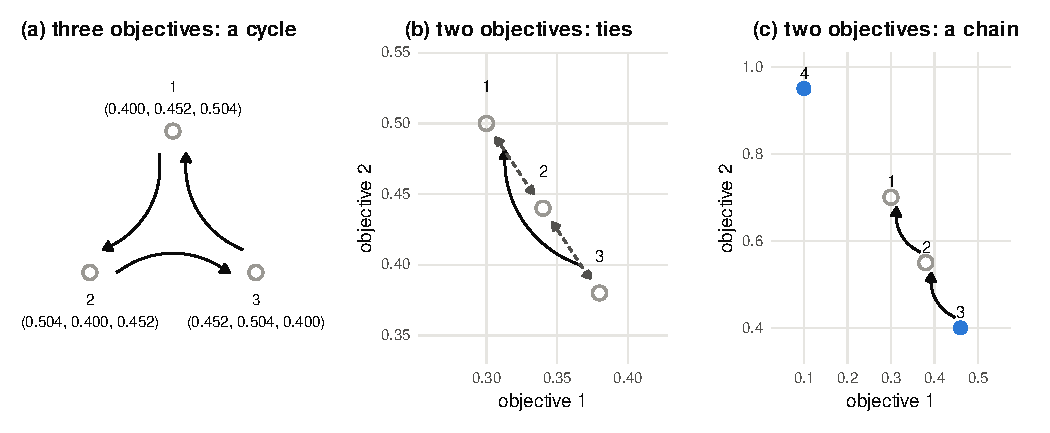
\includegraphics[width=\textwidth]{figures/fig1_failure.pdf}
\caption{The three instances of Proposition~\ref{prop:failure} with $\varepsilon=0.1$. Points are the mean vectors and arrows point from $j$ to $k$ when $j$ certifiably $\varepsilon$-dominates $k$; double-headed arrows are mutual certificates ($\varepsilon$-ties). (a) Three objectives, drawn in parallel coordinates: a cycle of one-directional certificates. (b) Two objectives: two ties and one one-directional certificate. (c) Two objectives: a chain $3\to2\to1$. Grey symbols are the alternatives that $\varepsilon$-elimination discards; in (a) and (b) it discards the whole Pareto set, which contains all alternatives. In all three panels, discarding by exact dominance discards nothing.}
\label{fig:failure}
\end{figure}

All three failures share a cause. A certificate that $j$ $\epsb$-dominates $k$ says something true about $j$ and $k$, but it is used to remove $k$ although nothing guarantees that $j$, or anything at least as good as $j$, will remain. Exact dominance does not have this defect: if $j$ certifiably dominates $k$ and $l$ certifiably dominates $j$, then $l$ certifiably dominates $k$, so the reason for a discard is never lost. The tolerance is still needed, but in the stopping rule rather than in the discarding rule. Proposition~\ref{prop:failure} does not depend on the confidence sequences, on the error level or on the allocation rule: it is a property of the decision rule applied to correct boxes. The simulation study in Section~\ref{sec:simulation} shows how often the failure occurs with noisy data.

\section{The procedure}\label{sec:method}

\subsection{Simultaneous confidence boxes}\label{sec:boxes}

For every alternative $k$ and objective $i$ we run a confidence sequence on the evaluations of $k$ alone. Let $N_k(t)$ be the number of evaluations of $k$ up to time $t$ and let $C_{k,i}(n)\subseteq[0,1]$ be the interval computed from the first $n$ evaluations of $k$ in objective $i$, at level $\alpha/(Km)$. Our default is the hedged betting confidence sequence of \citet[Theorem~3]{waudbysmith2024}. For a candidate mean $\theta$ it tracks the wealth of two gamblers who bet, with predictable stakes, that the observations exceed or fall short of $\theta$; $\theta$ is excluded when the hedged wealth reaches $Km/\alpha$. The sequence adapts to the variance without assuming a distributional family, which matters when an objective is a rare event or an average of many runs. The predictable plug-in Hoeffding and empirical Bernstein sequences of the same paper are also available. The box of $k$ at time $t$ is the running intersection
\[
B_k(t)=\prod_{i=1}^m\,[L_{k,i}(t),U_{k,i}(t)]=\prod_{i=1}^m\ \bigcap_{s\in T_t} C_{k,i}\{N_k(s)\},
\]
where $T_t\subseteq\{0,\dots,t\}$ is any set of times at which the intervals are computed; in the software, $T_t$ contains the end of every batch. Let $\Gev$ be the event that $\mub_k\in B_k(t)$ for all $k$ and all $t$.

\begin{lemma}\label{lem:boxes}
Under Assumption~A and any allocation rule, $\Prob(\Gev)\ge1-\alpha$.
\end{lemma}

\begin{proof}
Fix $k$, $i$ and $\theta=\mu_{k,i}$. The wealth of each gambler of alternative $k$, viewed in global time, is multiplied at time $t$ by $1+\lambda_t(X_{t,i}-\theta)$ if $A_t=k$ and by one otherwise, where the stake $\lambda_t$ is $\Fcal_{t-1}$-measurable and keeps the factor nonnegative. By Assumption~A the factor has conditional mean one, so each wealth process, and their convex combination (the hedged wealth), is a nonnegative martingale with initial value one. Ville's inequality \citep{ville1939} bounds by $\alpha/(Km)$ the probability that the hedged wealth ever reaches $Km/\alpha$, which is the only way in which $\theta$ can be excluded. The same argument applies to the Hoeffding and empirical Bernstein sequences. A union bound over the $Km$ sequences, and the fact that intersecting over any set of times cannot exclude a value that is never excluded, complete the proof.
\end{proof}

\subsection{Certificates}\label{sec:certificates}

At time $t$, write $\Lb_k$ and $\Ub_k$ for the corners of $B_k(t)$. We say that $j$ \emph{box-dominates} $k$, written $j\bdom k$, if $\Ub_j\le\Lb_k$ and $\Ub_j\ne\Lb_k$. The procedure reports the following sets:
\begin{align*}
\Dset_t&=\{k:\ j\bdom k\text{ for some }j\}\quad\text{(discarded)},\qquad \Sset_t=[K]\setminus\Dset_t\quad\text{(plausible)},\\
\Aset_t&=\{k\in\Sset_t:\ \text{for every } j\in\Sset_t\setminus\{k\}\text{ there is } i \text{ with } L_{j,i}>U_{k,i}-\varepsilon_i\}\quad\text{(accepted)},\\
\Cset_t&=\{k\in\Sset_t:\ \text{for every } j\in\Sset_t\setminus\{k\}\text{ there is } i \text{ with } L_{j,i}>U_{k,i}\}\quad\text{(certified optimal)},
\end{align*}
and a set of representatives $\Rset_t\subseteq\Sset_t$ such that for every $s\in\Sset_t$ there is $r\in\Rset_t$ with $\Ub_r\le\Lb_s+\epsb$; the software builds $\Rset_t$ greedily, adding at each step the plausible alternative that covers the largest number of uncovered ones. The acceptance condition says that no other plausible box reaches below the upper corner of $B_k(t)$ shifted by $-\epsb$ in every objective. By construction $\Cset_t\subseteq\Aset_t$, and the tolerance enters only $\Aset_t$ and $\Rset_t$.

\begin{lemma}\label{lem:order}
If $\Lb_k\le\Ub_k$ for every $k$, the relation $\bdom$ is irreflexive and transitive. Consequently every $k\in\Dset_t$ is box-dominated by some $s\in\Sset_t$.
\end{lemma}

\begin{proof}
Irreflexivity: $k\bdom k$ would require $\Ub_k\le\Lb_k$ with $\Ub_k\ne\Lb_k$, contradicting $\Lb_k\le\Ub_k$. Transitivity: if $l\bdom j$ and $j\bdom k$, then $\Ub_l\le\Lb_j\le\Ub_j\le\Lb_k$, and in a coordinate $i$ with $U_{j,i}<L_{k,i}$ we get $U_{l,i}<L_{k,i}$. A strict partial order on a finite set has no infinite descending chain, so following box-dominators from $k\in\Dset_t$ ends at a plausible alternative, which box-dominates $k$ by transitivity.
\end{proof}

\begin{theorem}\label{thm:validity}
On the event $\Gev$, simultaneously for all $t\ge0$:
\begin{enumerate}[label=(\roman*),leftmargin=*,itemsep=0pt]
\item every $k\in\Dset_t$ is dominated, $s\prec k$, by some plausible $s\in\Sset_t$, which the software reports;
\item $\Pset\subseteq\Sset_t$;
\item $\Aset_t\subseteq\Peps$;
\item every $k\in\Cset_t$ is Pareto-optimal, and no $j\ne k$ satisfies $\mub_j\le\mub_k$;
\item $\Rset_t$ $\epsb$-covers $\Pset$.
\end{enumerate}
Hence the probability that any of these statements is false at any time is at most $\alpha$, whatever the allocation rule and whenever the analyst stops. In particular, if $\tau$ is any stopping time with $\Aset_\tau=\Sset_\tau$, then $\widehat\Sset=\Sset_\tau$ satisfies the target~\eqref{eq:target} with probability at least $1-\alpha$.
\end{theorem}

\begin{proof}
On $\Gev$ every box contains its mean, so $\Lb_k\le\Ub_k$ and Lemma~\ref{lem:order} applies. (i) If $s\bdom k$, then $\mub_s\le\Ub_s\le\Lb_k\le\mub_k$, and in a coordinate with $U_{s,i}<L_{k,i}$ we have $\mu_{s,i}<\mu_{k,i}$; hence $s\prec k$. (ii) follows from (i). (iii) Let $k\in\Aset_t$ and suppose that $\mub_j\le\mub_k-\epsb$ for some $j\ne k$. If $j\in\Sset_t$, acceptance gives $i$ with $\mu_{j,i}\ge L_{j,i}>U_{k,i}-\varepsilon_i\ge\mu_{k,i}-\varepsilon_i$, a contradiction. If $j\in\Dset_t$, by (i) there is $s\in\Sset_t$ with $\mub_s\le\mub_j\le\mub_k-\epsb$, and $s\ne k$ because $s=k$ would give $\mub_k\le\mub_j\le\mub_k-\epsb$ together with $s\prec j$, which is impossible; the first case applied to $s$ gives the contradiction. (iv) The same argument with $\epsb=\bm0$ and weak inequalities. (v) For $p\in\Pset\subseteq\Sset_t$ there is $r\in\Rset_t$ with $\mub_r\le\Ub_r\le\Lb_p+\epsb\le\mub_p+\epsb$.
\end{proof}

Because the boxes are nested in time and the plausible set only shrinks, a certificate once issued is never withdrawn: $\Dset_t$ is nondecreasing, and an alternative that is accepted stays accepted while it is plausible. The report of an identification can therefore be audited at any time against its history.

\subsection{Allocation and stopping}\label{sec:allocation}

At time $t$, call a pair $(j,k)$ of distinct plausible alternatives \emph{open} if $j$ may still improve on $k$ by more than the tolerance without being certified to dominate it, that is, if neither $j\bdom k$ nor $L_{j,i}>U_{k,i}-\varepsilon_i$ for some $i$. A plausible alternative is accepted exactly when it is the second member of no open pair, so the identification ends when no pair is open. Closing an open pair requires the box of $j$, the box of $k$, or both, to shrink. The allocation rule evaluates both: among all alternatives that belong to an open pair, it evaluates $b$ times the one with the largest normalized width $w_k(t)=\max_i\{U_{k,i}(t)-L_{k,i}(t)\}$ per unit of evaluation cost (Algorithm~\ref{alg:procedure}).

\begin{algorithm}[t]
\spacingset{1}
\caption{Anytime-valid Pareto set identification}\label{alg:procedure}
\begin{algorithmic}[1]
\Require alternatives $[K]$, objectives with bounds, tolerance $\epsb$, level $\alpha$, batch size $b$, initial size $n_0$, costs $c_k$, budget
\State evaluate every alternative $n_0$ times; compute the boxes $B_k$
\While{some pair is open and the budget is not exhausted}
  \State $\mathcal{O}\gets\{a:\ a\text{ belongs to an open pair}\}$
  \State $a\gets\argmax_{a\in\mathcal{O}} w_a/c_a$ \Comment{ties broken by fewer evaluations}
  \State evaluate $a$ $b$ times; update its confidence sequences and intersect its box
\EndWhile
\State \Return $\Sset_t,\Aset_t,\Cset_t,\Dset_t$ with dominators, $\Rset_t$, boxes and history
\end{algorithmic}
\end{algorithm}

The choice of candidates is the second place where the obvious rule fails. If only alternatives whose status is undecided are evaluated, as in our first implementation, an accepted alternative $j$ whose wide box is the only obstacle to the acceptance or the discard of some $k$ is never evaluated again, and the pair $(j,k)$ remains open forever. Study~1 in Section~\ref{sec:simulation} shows this stalling in two of four configurations. With the open-pair rule the number of evaluations is bounded on $\Gev$. For distinct $j,k$ let
\[
d_{jk}=\min_i\,(\mu_{k,i}-\mu_{j,i}),\qquad a_{jk}=\max_i\,(\mu_{j,i}-\mu_{k,i}+\varepsilon_i),\qquad g_{jk}=\max(d_{jk},a_{jk}),
\]
the margins by which $j$ dominates $k$ and by which $j$ fails to improve on $k$ by the tolerance, and let $\Delta_k=\min_{j\ne k}\min(g_{jk},g_{kj})$. Since $a_{jk}\ge\varepsilon_{\min}-d_{jk}$ with $\varepsilon_{\min}=\min_i\varepsilon_i$, every gap satisfies $g_{jk}\ge\varepsilon_{\min}/2$.

\begin{theorem}\label{thm:termination}
Suppose $\varepsilon_{\min}>0$, all costs are equal, and on $\Gev$ the width of every box after $n$ evaluations satisfies $w_k\le w(n)$ for a nonincreasing function $w$ with $w(n)\to0$. Let $n^*(x)=\min\{n:w(n)<x\}$. Then on $\Gev$ the procedure of Algorithm~\ref{alg:procedure} stops after at most
\[
\sum_{k=1}^K\max\{n_0,\ n^*(\Delta_k/2)+b\}\ \le\ K\max\{n_0,\ n^*(\varepsilon_{\min}/4)+b\}
\]
evaluations.
\end{theorem}

\begin{proof}
On $\Gev$, $\Ub_j\le\mub_j+w_j$ and $\Lb_k\ge\mub_k-w_k$. If $w_j+w_k<d_{jk}$ then $U_{j,i}<L_{k,i}$ for every $i$, so $j\bdom k$; if $w_j+w_k<a_{jk}$ then $L_{j,i}>U_{k,i}-\varepsilon_i$ at the coordinate attaining $a_{jk}$. An open pair therefore has $w_j+w_k\ge g_{jk}$. When alternative $a$ is evaluated, it belongs to an open pair with some partner $c$, also a candidate, so $w_a\ge w_c$ and $2w_a\ge w_a+w_c\ge\Delta_a$. Thus $w(N_a)\ge\Delta_a/2$, so $N_a<n^*(\Delta_a/2)$ before each batch and $N_a<n^*(\Delta_a/2)+b$ after it.
\end{proof}

With unequal costs the same argument gives a bound that depends on the cost ratios. For the predictable plug-in Hoeffding sequence the width is deterministic and $n^*(x)=O\{x^{-2}\log(Km/\alpha)\log(1/x)(\log\log(1/x))^{2}\}$ (Section~\ref{S-sec:hoeffding} of the Supplementary Material), so the first bound has the form $\sum_k\Delta_k^{-2}\log(Km/\alpha)$ up to logarithmic factors, the form of the lower bound of \citet{auer2016}, whose gaps are defined differently. The second bound does not depend on the means: it is a budget, computable before the first evaluation, that suffices with probability at least $1-\alpha$ for every instance. With $\varepsilon_{\min}=0$ no such bound exists, because two alternatives with equal means can never be separated. For the betting sequence, whose width is random, we have no comparable bound.

\subsection{Practical aspects}\label{sec:practical}

An evaluation may be the average of several simulation runs; Assumption~A is preserved and fewer, less variable evaluations reduce the cost of the confidence sequences. Intervals are computed once per batch, which keeps the guarantee. The tolerance should be the smallest difference, in the units of each objective, that would change a decision; by Theorem~\ref{thm:validity} it determines when the procedure may stop but not what it may discard. The bounds $a_i,b_i$ must hold for every evaluation, and evaluations outside them are refused rather than clipped. The procedure is implemented in the R package \pkg{paretoinfer} \citep{paretoinfer}, which uses the confidence-sequence kernels of \pkg{seqbench} \citep{seqbench}; Section~\ref{S-sec:software} of the Supplementary Material shows the interface.

\section{Simulation study}\label{sec:simulation}

\subsection{Design}\label{sec:sim-design}

The study follows \citet{morris2019} and addresses hypotheses H1 to H3.

\paragraph{Data-generating mechanisms.} Every evaluation of alternative $k$ is a vector whose components have Beta distributions with means $\mu_{k,i}$ and concentration $\kappa$ (variance $\mu_{k,i}(1-\mu_{k,i})/(\kappa+1)$), coupled through a Gaussian copula with correlation $\rho$ between every pair of objectives. Study~1 uses six fixed configurations in which a wrong statement is easy to make: \emph{flat}, four Pareto-optimal alternatives with $m=2$, two of them closer than $\varepsilon=0.02$; \emph{close}, an alternative dominated by $0.03$ in both objectives next to three Pareto-optimal ones, $\varepsilon=0.02$, so that both a false discard and a false acceptance are possible; \emph{boundary}, an alternative dominated by exactly $\varepsilon=0.02$ in both objectives, which may be discarded but never accepted, next to three Pareto-optimal ones; \emph{cycle}, \emph{ties} and \emph{chain}, the instances of Proposition~\ref{prop:failure}(a), (b) and (c) with $\varepsilon=0.1$. The concentration is $\kappa=20$ in the first three and $\kappa=200$ in the last three. Study~2 draws a new instance in every replication: about half of the $K$ alternatives lie on the linear front $\sum_i\mu_{k,i}=\text{const}$ inside $[0.2,0.8]^m$, at points drawn uniformly on the simplex, and each of the others is a front point shifted upward by independent $U(0.02,0.15)$ amounts in every objective. The main grid crosses $K\in\{5,10,20\}$ with $\varepsilon\in\{0.025,0.05,0.10\}$ for $m=2$, $\kappa=20$ and $\rho=0$; secondary cells set $K=10$ and $\varepsilon=0.05$ and vary $m=3$, $\rho=\pm0.6$, or the confidence sequence.

\paragraph{Methods.} All methods use $\alpha=0.05$, an initial batch of $n_0=5$ evaluations per alternative and batches of $b=5$. The proposed procedure (Algorithm~\ref{alg:procedure}, betting sequences on a grid of 1001 points without endpoint refinement) is compared with three variants that each change one ingredient: $\varepsilon$-elimination with the tie-break and the allocation of our first implementation (``$\varepsilon$-discarding''); fixed-sample Student-$t$ intervals recomputed after every batch, at the same split level $\alpha/(Km)$ (``repeated $t$''); and betting sequences at level $\alpha$ each, without the union bound (``no correction''). Study~2 also compares the open-pair allocation with uniform allocation, which evaluates every plausible alternative in turn. The budget is $10^4$ evaluations in Study~1 and $3\times10^4$ in Study~2.

\paragraph{Performance measures.} After every batch, every statement of Theorem~\ref{thm:validity} is checked against the true means: a discarded alternative that is not dominated, an accepted alternative outside $\Peps$, a certified-optimal alternative outside $\Pset$, and, at the end, representatives that fail to $\epsb$-cover $\Pset$. A replication counts as an \emph{error} if any of these occurs at any time. For $\varepsilon$-discarding the corresponding statement is that each discarded alternative is truly $\epsb$-dominated. For all methods we record \emph{frontier loss}, the event that the plausible set fails to $\epsb$-cover $\Pset$ at some time, which is the common target of all methods. We also record the number of evaluations and whether the identification ended before the budget. Study~1 uses 200 replications per cell, so that an error rate of $0.05$ is estimated with a Monte Carlo standard error of about $0.015$; Study~2 uses 30 replications per cell.

\subsection{Results}\label{sec:sim-results}

\paragraph{Validity (Study~1).} Table~\ref{tab:validity} reports, for each configuration and method, the percentage of replications with an error and with frontier loss and the median number of evaluations. The proposed procedure made no false statement in any of the 1200 replications and always stopped. $\varepsilon$-discarding lost the Pareto set in every replication of the cycle configuration and in 1.5\% of the chain configuration. In the tie configuration it lost nothing: the certificates $2\to1$ and $3\to2$ have larger margins than the ties of Proposition~\ref{prop:failure}(b) and appear first, so alternative~3 survives alone and covers the other two. Its allocation, which evaluates only undecided alternatives, did not stop within $10^4$ evaluations in the flat, close and chain configurations, the stalling discussed in Section~\ref{sec:allocation}. Repeated $t$ intervals stopped earliest and were the only method to err, in 3.5\% of the replications of the close configuration (95\% Clopper--Pearson interval 1.4\% to 7.1\%); this rate is below the nominal level, and the configurations were not adverse enough to push it above. In the boundary configuration no method erred, and the proposed procedure needed a median of 4982 evaluations, against 1555 for repeated $t$ intervals and 3322 without the union bound, which is the price of validity in this configuration. Confidence sequences without the union bound made no error, which we discuss in Section~\ref{sec:discussion}.

\begin{table}[tbp]
\spacingset{1}
\centering
\caption{Study~1: percentage of the 200 replications with an error (Err.) and with frontier loss (Loss), and median number of evaluations (Eval.); in parentheses, the percentage that stopped within $10^4$ evaluations when below 100. With 200 replications, the upper 95\% Clopper--Pearson limit for an observed rate of zero is 1.8\%.}
\label{tab:validity}
\footnotesize
\begin{tabular}{llrrrr}
\toprule
Configuration & Method & Error (\%) & Frontier loss (\%) & Stopped (\%) & Evaluations \\
\midrule
flat & proposed & 0.0 (0.0, 1.8) & 0.0 (0.0, 1.8) & 100 & 1390 \\
 & $\varepsilon$-discarding & 0.0 (0.0, 1.8) & 0.0 (0.0, 1.8) & 0 & 10000 \\
 & repeated $t$ & 0.0 (0.0, 1.8) & 0.0 (0.0, 1.8) & 100 & 532 \\
 & no correction & 0.0 (0.0, 1.8) & 0.0 (0.0, 1.8) & 100 & 935 \\
\addlinespace
close & proposed & 0.0 (0.0, 1.8) & 0.0 (0.0, 1.8) & 100 & 3268 \\
 & $\varepsilon$-discarding & 0.0 (0.0, 1.8) & 0.0 (0.0, 1.8) & 0 & 10000 \\
 & repeated $t$ & 3.5 (1.4, 7.1) & 0.5 (0.0, 2.8) & 100 & 1260 \\
 & no correction & 0.0 (0.0, 1.8) & 0.0 (0.0, 1.8) & 100 & 2185 \\
\addlinespace
boundary & proposed & 0.0 (0.0, 1.8) & 0.0 (0.0, 1.8) & 99 & 4982 \\
 & $\varepsilon$-discarding & 0.0 (0.0, 1.8) & 0.0 (0.0, 1.8) & 100 & 1390 \\
 & repeated $t$ & 0.0 (0.0, 1.8) & 0.0 (0.0, 1.8) & 100 & 1555 \\
 & no correction & 0.0 (0.0, 1.8) & 0.0 (0.0, 1.8) & 100 & 3322 \\
\addlinespace
cycle & proposed & 0.0 (0.0, 1.8) & 0.0 (0.0, 1.8) & 100 & 225 \\
 & $\varepsilon$-discarding & 0.0 (0.0, 1.8) & 100.0 (98.2, 100.0) & 100 & 730 \\
 & repeated $t$ & 0.0 (0.0, 1.8) & 0.0 (0.0, 1.8) & 100 & 20 \\
 & no correction & 0.0 (0.0, 1.8) & 0.0 (0.0, 1.8) & 100 & 145 \\
\addlinespace
ties & proposed & 0.0 (0.0, 1.8) & 0.0 (0.0, 1.8) & 100 & 230 \\
 & $\varepsilon$-discarding & 0.0 (0.0, 1.8) & 0.0 (0.0, 1.8) & 100 & 545 \\
 & repeated $t$ & 0.0 (0.0, 1.8) & 0.0 (0.0, 1.8) & 100 & 20 \\
 & no correction & 0.0 (0.0, 1.8) & 0.0 (0.0, 1.8) & 100 & 155 \\
\addlinespace
chain & proposed & 0.0 (0.0, 1.8) & 0.0 (0.0, 1.8) & 100 & 230 \\
 & $\varepsilon$-discarding & 0.0 (0.0, 1.8) & 1.5 (0.3, 4.3) & 2 & 10000 \\
 & repeated $t$ & 0.0 (0.0, 1.8) & 0.0 (0.0, 1.8) & 100 & 20 \\
 & no correction & 0.0 (0.0, 1.8) & 0.0 (0.0, 1.8) & 100 & 150 \\
\bottomrule
\end{tabular}

\end{table}

\paragraph{Efficiency (Study~2).} No method made a false statement in Study~2 (Figure~\ref{fig:efficiency}). The open-pair allocation needed fewer evaluations than uniform allocation in every cell of the main grid, with median savings between 18\% and 44\%; the saving was largest for $\varepsilon=0.05$ and smallest for $\varepsilon=0.10$, and it did not increase with $K$. The number of evaluations grew faster than in proportion to $K$ and much less than in proportion to $\varepsilon^{-2}$. $\varepsilon$-discarding with its own allocation stopped in a proportion of replications that fell with $K$ and with smaller tolerances, and with $K=20$ and $\varepsilon=0.10$ it lost part of the Pareto set in 43\% of the replications. In the secondary cells, three objectives raised the median from 3613 to 5018 evaluations (7835 with uniform allocation), correlations of $\pm0.6$ raised it to about 4000, the empirical-Bernstein sequence needed 6455, and the Hoeffding sequence did not stop within $3\times10^4$ evaluations in any replication. Table~\ref{S-tab:study2} of the Supplementary Material gives all cells.

\begin{figure}[t]
\spacingset{1}
\centering
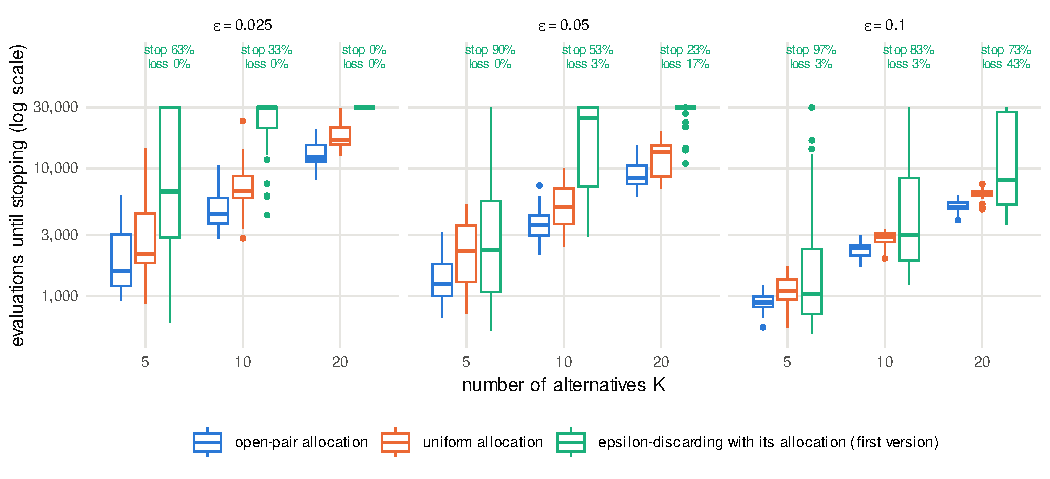
\includegraphics[width=0.92\textwidth]{figures/fig2_efficiency.pdf}
\caption{Study~2: number of evaluations until stopping, 30 random instances per box, $m=2$, $\rho=0$. Boxes for $\varepsilon$-discarding include replications censored at $3\times10^4$; the labels give the percentage that stopped and the percentage with frontier loss.}
\label{fig:efficiency}
\end{figure}


\section{Applications}\label{sec:applications}

Both applications use the public interface of the software with $\alpha=0.05$, betting sequences with endpoint refinement, $n_0=b=5$, the optional cover phase described below, and a budget of $10^5$ evaluations. In both the true means can be computed exactly, so that each statement can be checked.

\subsection{Interval estimators for a binomial proportion}\label{sec:app-binomial}

Simulation studies of interval estimators report average coverage and length from a fixed number of replications \citep{morris2019}. We compare eight 95\% intervals for a binomial proportion with $n=30$: Wald, Wilson, Wilson with continuity correction (Wilson-cc), Agresti--Coull, Clopper--Pearson, Jeffreys, arcsine and likelihood ratio \citep{clopper1934,newcombe1998,agresti1998,brown2001}. The two objectives are the miscoverage and the width, averaged over $p\sim U(0,1)$. Both are bounded by $[0,1]$ and the truth is exact: given $X=x$, $p$ has a Beta$(x+1,n-x+1)$ distribution and $\Prob(X=x)=1/(n+1)$, so each method's average coverage is a finite sum of incomplete beta functions. Seven of the eight methods are Pareto-optimal; Wilson-cc is dominated by Clopper--Pearson by $0.0004$ in miscoverage and $0.0008$ in width (Table~\ref{S-tab:binomial} in the Supplementary Material). One evaluation is the average, over 100 simulated studies, of the miscoverage indicator and the width, and the tolerance is $0.005$ in both objectives, half a percentage point of coverage and $0.005$ in width.

All eight methods were accepted after 20{,}130 evaluations, that is, about $2\times10^6$ simulated studies (Figure~\ref{fig:applications}a). Five were certified optimal and three, Wilson-cc, Clopper--Pearson and likelihood ratio, were accepted as $\epsb$-Pareto-optimal; none was discarded, which is correct, because the only dominated method is dominated by much less than the tolerance. Deciding a difference of $0.0004$ in miscoverage would require intervals far narrower than any practical question needs. Since every method was accepted, the accepted set says little; the representatives say more. At acceptance they coincided with the plausible set, because the boxes were too wide to certify any cover. In the cover phase, which evaluates pairs of plausible alternatives until it is certified whether one $\epsb$-covers the other, they fell to four methods: Wald, Wilson, Agresti--Coull and Wilson-cc. Every Pareto-optimal method is therefore within $0.005$ in both objectives of one of these four, with probability at least $0.95$. The cover phase did not finish within the budget: eight ordered pairs remained undecided, and in each of them the true cover margin, the amount by which one method fails to be within $\epsb$ of the other or succeeds, is below $0.002$. This is the case that Theorem~\ref{thm:termination} does not reach. The usual table of estimated coverages and widths suggests a summary of this kind; the cover certifies it.

\subsection{Reorder policies for an inventory system}\label{sec:app-inventory}

The second application is a periodic-review $(s,S)$ inventory system with backlogging, modelled after the example of \citet[Section~1.5]{law2015}. Demand in each period is Binomial$(50,1/2)$; at the end of a period with inventory level $I<s$ an order of $S-I$ units is placed and arrives at the start of the next period. Each period costs 32 per order plus 3 per unit ordered, 1 per unit held and 5 per unit short. One evaluation is a replication of 60 periods after a warm-up of 20, and the two objectives are the average cost per period and the fraction of periods that end with a backlog. The $K=16$ policies cross $s\in\{10,20,30,40\}$ with $S-s\in\{20,40,60,80\}$. Because demand is bounded, the cost lies in $[0,832]$, a range about six times wider than the costs observed, and the backlog fraction in $[0,1]$; the two are correlated within a replication (about $0.5$). The level at the start of a period is a Markov chain on $\{s,\dots,S\}$, so both objectives are finite sums that we compute exactly; four policies are Pareto-optimal, all with $S-s=40$ (Table~\ref{S-tab:inventory}). The tolerance is one unit of cost and half a percentage point of backlog.

Every plausible policy was accepted after 59{,}510 evaluations (Figure~\ref{fig:applications}b). Seven policies were discarded, each with a plausible dominator named in the report; three were certified optimal; and six were accepted as $\epsb$-Pareto-optimal. Five of these six are dominated, among them $(40,100)$, which costs $3.8$ more per period than $(40,80)$ and, like it, runs out of stock in fewer than one period in $10^7$. We had not anticipated this when we chose the tolerance, but it follows from the definition: an alternative is $\epsb$-Pareto-optimal unless another improves on it by at least $\epsb$ in \emph{every} objective, and no policy can improve by $0.005$ on a backlog fraction below $0.005$. An alternative within $\varepsilon_i$ of the lower bound of objective $i$ is therefore never excluded by the target~\eqref{eq:target}, however large its disadvantage in the others. The representatives correct this: after the cover phase they are the three policies $(10,50)$, $(20,60)$ and $(30,70)$, which $\epsb$-cover the four Pareto-optimal policies; $(40,80)$ is represented by $(30,70)$, which costs $10$ less per period and runs out of stock in $0.05\%$ of periods. Here too the budget ended in the cover phase, with two pairs among the policies with $s\ge30$ undecided; neither involves a representative. The loose bound on cost was not costly because the betting sequences adapt to the small variance of the cost.

\begin{figure}[t]
\spacingset{1}
\centering
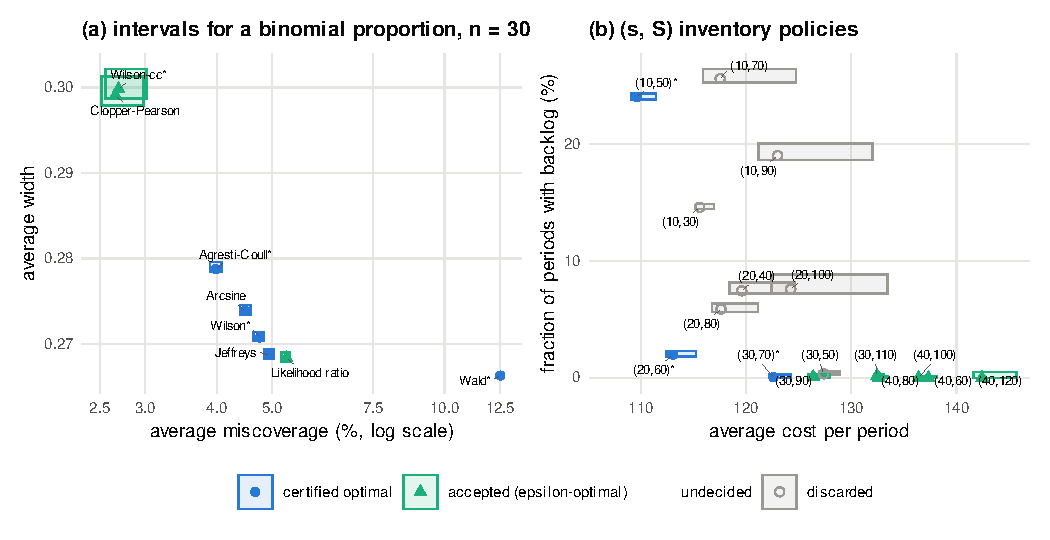
\includegraphics[width=\textwidth]{figures/fig3_applications.pdf}
\caption{The two applications at the end of one identification. Rectangles are the simultaneous confidence boxes, points are the true mean vectors, colour and shape give the status, and an asterisk marks the representatives. (a) Eight intervals for a binomial proportion with $n=30$; miscoverage on a logarithmic scale. (b) Sixteen $(s,S)$ inventory policies; the horizontal axis is restricted to the range of the boxes of the plausible policies.}
\label{fig:applications}
\end{figure}

To check the statements against the truth, each identification was repeated %APPREP% times with independent random numbers. %APPREPRESULT%

\section{Discussion}\label{sec:discussion}

The hypotheses of Section~\ref{sec:intro} received different degrees of support. H1 was supported where Proposition~\ref{prop:failure} predicts it: $\varepsilon$-elimination lost the Pareto set in every replication of the cycle and in some replications of the chain, but not in the tie configuration, where the certificates that create the cycle appear in an order the procedure never reaches. The failure depends on the configuration and can pass a test suite unnoticed. H2 was supported for the proposed procedure, which made no false statement in any replication, but not for the comparison: repeated $t$ intervals erred in one configuration at a rate below $\alpha$, and confidence sequences without a correction did not err. What separates these methods in our studies is the guarantee, not the observed error rate. H3 was supported in direction only: the open-pair allocation saved evaluations in every cell, but the saving did not grow with $K$.

Without the union bound no error occurred because a false statement requires a sequence to fail in the direction that changes a certificate, when that certificate is decided, and only a few of the $Km$ sequences matter; the union bound protects against all failures and is conservative. Its cost is moderate, since widths grow with $\log(Km/\alpha)$: with $K=20$, $m=2$ and $\alpha=0.05$ it replaces $\log 20\approx3.0$ by $\log 800\approx6.7$. A sharper correction would have to use the correlation between objectives, which in Study~2 changed the number of evaluations by 10 to 15\%; rules for combining e-values \citep{vovk2021} are a possible route.

The budget of Theorem~\ref{thm:termination} is valid for every instance but is not a planning tool: for $K=10$, $m=2$ and $\varepsilon=0.05$ the Hoeffding sequence requires about $4.6\times10^6$ evaluations (Table~\ref{S-tab:horizon}), more than a thousand times the median used by the betting sequence in Study~2, for which we have no comparable bound. A pilot identification is a better guide, and, being anytime-valid, it is not wasted.

The setting has two limitations. First, the bounds of every objective must be known and must hold. For averages of indicators and other bounded measures they do; for costs or response times without a natural ceiling the analyst must justify a bound or transform the objective. In the inventory application a bound six times wider than the observed range cost little, but only because the betting sequence adapts to the variance. Second, evaluations of different alternatives are treated as independent, so common random numbers, which in ranking and selection often reduce the number of replications substantially \citep{hunter2019}, are not exploited. Anytime-valid sequences for paired differences exist \citep{seqbench}, and certificates built on differences would combine both ideas, at the price of $K(K-1)m/2$ sequences instead of $Km$.

The applications showed a property of the target that we had not anticipated: an alternative within $\varepsilon_i$ of the lower bound of objective $i$ is $\epsb$-Pareto-optimal whatever its other values, and five dominated inventory policies were accepted for this reason. The certified cover removes them, but its phase is more expensive and its last pairs, whose cover margins are near zero, did not resolve within the budget; Theorem~\ref{thm:termination} does not cover this phase. We regard $\Peps$ as a stopping criterion and the cover as the description of the frontier.

\subsection{Conclusions}\label{sec:conclusion}

Identifying the Pareto set from noisy simulations involves two decisions that the usual procedures merge: what to discard and when to stop. We separated them. Discarding uses only exact dominance certified by simultaneous confidence boxes, so it never loses a Pareto-optimal alternative; the tolerance enters only the decision to accept, and a certified cover summarizes the result. The statements hold with probability at least $1-\alpha$ simultaneously over time, under any allocation and at any stopping time. %CONCLNUM% The price is the need for known bounds and the conservativeness of the union bound; the gain is that every intermediate report, including the one produced when the budget runs out, is a valid statement about the alternatives.


\bigskip
\begin{center}
{\large\bf SUPPLEMENTARY MATERIAL}
\end{center}
\begin{description}[leftmargin=*]
\item[Supplement:] proofs of Proposition~\ref{prop:failure} and of the asymptotic width of the Hoeffding sequence, planning horizons, software interface, details of the applications and additional simulation results (PDF).
\item[Code and data:] R scripts that reproduce every number, table and figure, and the version of the R package used (archive).
\end{description}


\spacingset{1}
\bibliographystyle{agsm}
\bibliography{refs}

\end{document}
